%%%%%%%%%%%%%%%%%%%%%%%%%%%%%%%%%%%%%%%%%
% Lachaise Assignment
% LaTeX Template
% Version 1.0 (26/6/2018)
%
% This template originates from:
% http://www.LaTeXTemplates.com
%
% Authors:
% Marion Lachaise & François Févotte
% Vel (vel@LaTeXTemplates.com)
%
% License:
% CC BY-NC-SA 3.0 (http://creativecommons.org/licenses/by-nc-sa/3.0/)
% 
%%%%%%%%%%%%%%%%%%%%%%%%%%%%%%%%%%%%%%%%%



%----------------------------------------------------------------------------------------
%	PACKAGES AND OTHER DOCUMENT CONFIGURATIONS
%----------------------------------------------------------------------------------------

\documentclass{article}

\usepackage{dirtree}

\usepackage{hyperref}

%%%%%%%%%%%%%%%%%%%%%%%%%%%%%%%%%%%%%%%%%
% Lachaise Assignment
% Structure Specification File
% Version 1.0 (26/6/2018)
%
% This template originates from:
% http://www.LaTeXTemplates.com
%
% Authors:
% Marion Lachaise & François Févotte
% Vel (vel@LaTeXTemplates.com)
%
% License:
% CC BY-NC-SA 3.0 (http://creativecommons.org/licenses/by-nc-sa/3.0/)
% 
%%%%%%%%%%%%%%%%%%%%%%%%%%%%%%%%%%%%%%%%%

%----------------------------------------------------------------------------------------
%	PACKAGES AND OTHER DOCUMENT CONFIGURATIONS
%----------------------------------------------------------------------------------------

\usepackage{amsmath,amsfonts,stmaryrd,amssymb} % Math packages

\usepackage{enumerate} % Custom item numbers for enumerations

\usepackage[ruled]{algorithm2e} % Algorithms

\usepackage[framemethod=tikz]{mdframed} % Allows defining custom boxed/framed environments

\usepackage{listings} % File listings, with syntax highlighting
\lstset{
	basicstyle=\ttfamily, % Typeset listings in monospace font
}

%----------------------------------------------------------------------------------------
%	DOCUMENT MARGINS
%----------------------------------------------------------------------------------------

\usepackage{geometry} % Required for adjusting page dimensions and margins

\geometry{
	paper=a4paper, % Paper size, change to letterpaper for US letter size
	top=2.5cm, % Top margin
	bottom=3cm, % Bottom margin
	left=2.5cm, % Left margin
	right=2.5cm, % Right margin
	headheight=14pt, % Header height
	footskip=1.5cm, % Space from the bottom margin to the baseline of the footer
	headsep=1.2cm, % Space from the top margin to the baseline of the header
	%showframe, % Uncomment to show how the type block is set on the page
}

%----------------------------------------------------------------------------------------
%	FONTS
%----------------------------------------------------------------------------------------

\usepackage[utf8]{inputenc} % Required for inputting international characters
\usepackage[T1]{fontenc} % Output font encoding for international characters

\usepackage{XCharter} % Use the XCharter fonts

%----------------------------------------------------------------------------------------
%	COMMAND LINE ENVIRONMENT
%----------------------------------------------------------------------------------------

% Usage:
% \begin{commandline}
%	\begin{verbatim}
%		$ ls
%		
%		Applications	Desktop	...
%	\end{verbatim}
% \end{commandline}

\mdfdefinestyle{commandline}{
	leftmargin=10pt,
	rightmargin=10pt,
	innerleftmargin=15pt,
	middlelinecolor=black!50!white,
	middlelinewidth=2pt,
	frametitlerule=false,
	backgroundcolor=black!5!white,
	frametitle={Command Line},
	frametitlefont={\normalfont\sffamily\color{white}\hspace{-1em}},
	frametitlebackgroundcolor=black!50!white,
	nobreak,
}

% Define a custom environment for command-line snapshots
\newenvironment{commandline}{
	\medskip
	\begin{mdframed}[style=commandline]
}{
	\end{mdframed}
	\medskip
}

%----------------------------------------------------------------------------------------
%	FILE CONTENTS ENVIRONMENT
%----------------------------------------------------------------------------------------

% Usage:
% \begin{file}[optional filename, defaults to "File"]
%	File contents, for example, with a listings environment
% \end{file}

\mdfdefinestyle{file}{
	innertopmargin=1.6\baselineskip,
	innerbottommargin=0.8\baselineskip,
	topline=false, bottomline=false,
	leftline=false, rightline=false,
	leftmargin=2cm,
	rightmargin=2cm,
	singleextra={%
		\draw[fill=black!10!white](P)++(0,-1.2em)rectangle(P-|O);
		\node[anchor=north west]
		at(P-|O){\ttfamily\mdfilename};
		%
		\def\l{3em}
		\draw(O-|P)++(-\l,0)--++(\l,\l)--(P)--(P-|O)--(O)--cycle;
		\draw(O-|P)++(-\l,0)--++(0,\l)--++(\l,0);
	},
	nobreak,
}

% Define a custom environment for file contents
\newenvironment{file}[1][File]{ % Set the default filename to "File"
	\medskip
	\newcommand{\mdfilename}{#1}
	\begin{mdframed}[style=file]
}{
	\end{mdframed}
	\medskip
}

%----------------------------------------------------------------------------------------
%	NUMBERED QUESTIONS ENVIRONMENT
%----------------------------------------------------------------------------------------

% Usage:
% \begin{question}[optional title]
%	Question contents
% \end{question}

\mdfdefinestyle{question}{
	innertopmargin=1.2\baselineskip,
	innerbottommargin=0.8\baselineskip,
	roundcorner=5pt,
	nobreak,
	singleextra={%
		\draw(P-|O)node[xshift=1em,anchor=west,fill=white,draw,rounded corners=5pt]{%
		Question \theQuestion\questionTitle};
	},
}

\newcounter{Question} % Stores the current question number that gets iterated with each new question

% Define a custom environment for numbered questions
\newenvironment{question}[1][\unskip]{
	\bigskip
	\stepcounter{Question}
	\newcommand{\questionTitle}{~#1}
	\begin{mdframed}[style=question]
}{
	\end{mdframed}
	\medskip
}

%----------------------------------------------------------------------------------------
%	WARNING TEXT ENVIRONMENT
%----------------------------------------------------------------------------------------

% Usage:
% \begin{warn}[optional title, defaults to "Warning:"]
%	Contents
% \end{warn}

\mdfdefinestyle{warning}{
	topline=false, bottomline=false,
	leftline=false, rightline=false,
	nobreak,
	singleextra={%
		\draw(P-|O)++(-0.5em,0)node(tmp1){};
		\draw(P-|O)++(0.5em,0)node(tmp2){};
		\fill[black,rotate around={45:(P-|O)}](tmp1)rectangle(tmp2);
		\node at(P-|O){\color{white}\scriptsize\bf !};
		\draw[very thick](P-|O)++(0,-1em)--(O);%--(O-|P);
	}
}

% Define a custom environment for warning text
\newenvironment{warn}[1][Warning:]{ % Set the default warning to "Warning:"
	\medskip
	\begin{mdframed}[style=warning]
		\noindent{\textbf{#1}}
}{
	\end{mdframed}
}

%----------------------------------------------------------------------------------------
%	INFORMATION ENVIRONMENT
%----------------------------------------------------------------------------------------

% Usage:
% \begin{info}[optional title, defaults to "Info:"]
% 	contents
% 	\end{info}

\mdfdefinestyle{info}{%
	topline=false, bottomline=false,
	leftline=false, rightline=false,
	nobreak,
	singleextra={%
		\fill[black](P-|O)circle[radius=0.4em];
		\node at(P-|O){\color{white}\scriptsize\bf i};
		\draw[very thick](P-|O)++(0,-0.8em)--(O);%--(O-|P);
	}
}

% Define a custom environment for information
\newenvironment{info}[1][Info:]{ % Set the default title to "Info:"
	\medskip
	\begin{mdframed}[style=info]
		\noindent{\textbf{#1}}
}{
	\end{mdframed}
}
 % Include the file specifying the document structure and custom commands


%----------------------------------------------------------------------------------------
%	ASSIGNMENT INFORMATION
%----------------------------------------------------------------------------------------

\title{The Foodie Web Service Project\\ } % Title of the assignment

%\author{David Domingo\\ \texttt{djd240@cs.rutgers.edu}} % Author name and email address

%\author{Rutgers University} % Author name and email address

%\date{Due: Some Date, 11:55pm} % University, school and/or department name(s) and a date
\date{} %empty date

%----------------------------------------------------------------------------------------

\begin{document}

\maketitle % Print the title

%----------------------------------------------------------------------------------------
%	INTRODUCTION
%----------------------------------------------------------------------------------------

\section*{Introduction} % Unnumbered section

In this project we will be exploring RESTful web services. Every day we interact with web services in everything we do, on our phone, on our computers, Google Maps, Twitter, Facebook, you name it. Behind every service you use, are many systems interacting with each other to provide you with a service that is seamless. This is a distributed system! In this project we'll be creating our own distributed system for food lovers. We'll be creating a simple Web Service that will take an address and respond with info of nearby restaurants. In order for our service to provide such functionality, we'll have to coordinate and interact with other web services to get data that we'll need to give our client what they want.

%----------------------------------------------------------------------------------------
%	Background
%----------------------------------------------------------------------------------------

\section*{Background}

\subsection*{Intro to RESTful Design}
RESTful design is a popular architectural style in today's world of distributed systems. REST stand for "Representational State Transfer".  RESTful design helps make communication between systems be stateless. A RESTful service is simply a server that provides access to resources. Each resource is identified by URIs/Global IDs. Clients can then interact with the resources by sending HTTP requests to a service's RESTful API which is a collection of service endpoints that allows some form of interaction with a resource. In the end, RESTful design allow for systems to easily communicate and interact with resources through HTTP requests.

\-\\\ Learn more about RESTful Design and REST APIs here:
\begin{itemize}
\item REST API concepts and examples - https://youtu.be/7YcW25PHnAA 
\item What is a RESTful API? Explanation of REST and HTTP - https://youtu.be/Q-BpqyOT3a8
\item \href{https://www.cs.rutgers.edu/~pxk/417/notes/content/03r-recitation.pdf}{https://www.cs.rutgers.edu/~pxk/417/notes/content/03r-recitation.pdf}
\end{itemize}

\begin{info}[Recommended video:]
I highly recommend watching the first video "REST API concepts and examples". It has a great explanation of how RESTful services and RESTful APIs work as well as give a brief overview of HTTP/JSON. This should give you a general overview of the concepts you will need to know for this project.
\end{info}

\subsection*{Intro to HTTP Requests}
In order to carry out RESTful calls you will need to understand Hypertext Transfer Protocol (HTTP), which at the heart of RESTful architecture. Typically services use HTTP to communicate with each  other and carry out "RESTful" calls. HTTP Requests have a particular format. There are multiple types HTTP methods, including GET, POST, PUT, PATCH, DELETE. There are other methods, but these are the basic ones that are used. These methods give the server an idea of what kind of operations the client wants to perform on a resource. For example, every time you go to a website on your web browser, your web browser sends a GET request to the server, letting it know that it wants to get a resource, with the resource being a webpage in this case. HTTP requests can pass information to a service through request parameters and/or request headers. For example, typically HTTP requests have header called "Content-Type" that passes information about the format of the request body.  Now as a result of a HTTP request you will get a response. An HTTP response has a similar format to a HTTP request and can pass information back to the client by setting response parameters, headers, or the body. The only difference is that an HTTP response also has a number known as a status code. A status code gives the client about some insight on how the request was handled. For example, in most cases, when a request is successfully processed, the response usually has the status code of 200 which represents success. 

\-\\\ Read more about HTTP here:
\begin{itemize}
\item HTTP Quick Guide - https://www.tutorialspoint.com/http/http\_quick\_guide.htm
\item What is a RESTful API? Explanation of REST and HTTP - https://youtu.be/Q-BpqyOT3a8
\item HTTP Status Codes - https://www.restapitutorial.com/httpstatuscodes.html
\end{itemize}

\subsection*{Intro to JSON}
The most popular way to serialize and pass data within HTTP requests is with JSON objects. When working with REST APIs, you will most likely see information being returned in JSON format. JSON stands for JavaScript Object Notation. JSON is a human-readable format and consists of key/value pairs. In this project you will be receiving responses in JSON from API requests as well as sending JSON back to the client, so it is important to understand the JSON formate and how to handle JSON with the particular programming language/framework that you choose to use. 

\-\\\ Read more about JSON here:
\begin{itemize}
\item Introducing JSON - https://www.json.org/
\item JSON Simple Wiki - https://simple.wikipedia.org/wiki/JSON
\end{itemize}


%----------------------------------------------------------------------------------------
%	Architecture and Flow
%----------------------------------------------------------------------------------------
\section*{The Foodie WebService}
Your task is to build the back-end of our Foodie Web Service. We want the web service to take a HTTP request with an address parameter and respond with a list popular restaurants nearby. How will we do this? Fortunately we have two APIs that we can use to do just that. Geocod.io is a Geocoding web service that can take an address and turn it into a geographic description (e.g. latitude and longitude). Zomato is a web service that provides restaurant content and has a REST endpoint that can find a nearby restaurants given latitude and longitude as input. We'll use both of these services we can create our Foodie Web Service.

\begin{figure}[h!]
 \centering
 
\includegraphics[width=60mm]{images/geocodio}
 
\includegraphics[width=60mm]{images/Zomato}
\end{figure} 

\section*{Architecture and Flow}
In figure 1 you can see the main architecture of our web service. Our web service will consist of three systems: (1) our foodie web service that will handle requests, (2) the Geocod.io web service that will geocode an address, and (3) the Zomato web service that will find nearby restaurants.


\-\ \\
The flow of handling a client request to our /restaurants endpoint can seen in figure 2. As you'll see, our client will send a request with an address to our web service. Our web service will then take that address, geocode that address by making a API call to Geocod.io, then find nearby restaurants by making a second API call to Zomato with our geocoded address. In this case, a client could be a web page, an app on a phone, or even another web service, but in this project we will only be focussing on the web service. You will not need to implement your own client. We will be using HTTP request tools to act as a client.  \\\\

\begin{figure}[h!]
    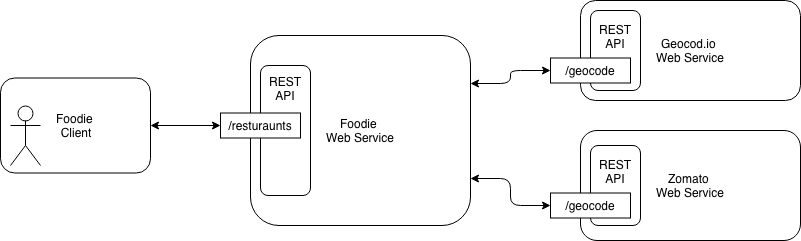
\includegraphics[width=\linewidth]{images/architecture}
    \caption{Architecture of the Foodie Web Service}
\end{figure}


\begin{figure}[h!]
    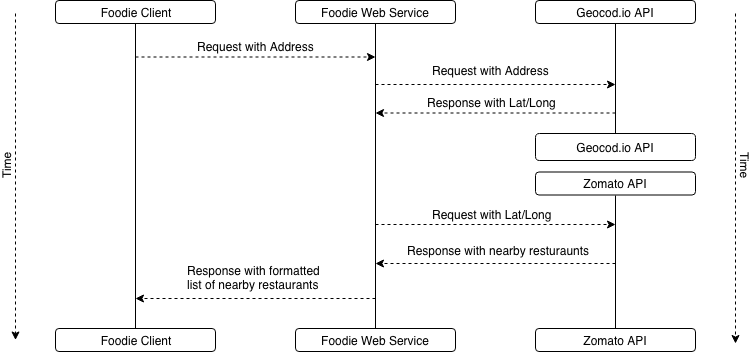
\includegraphics[width=\linewidth]{images/flowdiagram}
    \caption{Flow Diagram of the Foodie Web Service}
\end{figure}




%----------------------------------------------------------------------------------------
%	Project Stages
%----------------------------------------------------------------------------------------

\section*{Project Stages} % Numbered section

To implement our Foodie Web Service, we will break down this project into six stages:
\begin{itemize}  
\item Stage 1 - Starting a RESTful Web Service
\item Stage 2 - Passing Some Input
\item Stage 3 - Geocoding our Address
\item Stage 4 - Finding Nearby Restaurants
\item Stage 5 - Formatting Client Responses
\item Stage 6 - Fault Tolerance
\end{itemize}


%----------------------------------------------------------------------------------------
%	Stage 1
%----------------------------------------------------------------------------------------

\section{Starting a RESTful Web service}
The first part of this project to start off by creating the base of your RESTful webs service. Here you can use the following languages and the corresponding frameworks:
\begin{itemize}
\item Java (Spring)
\item Javascript (Node.js/Express)
\item Python (Flask/Django)
\end{itemize}
There are many tutorials out there to help you get started making a RESTful web service. Some links will be provided in the Resources section of this document. 

\-\\\ Using these frameworks we want to make a web service with a single REST endpoint:
\begin{itemize}
\item /restaurants - Returns list of nearby restaurants given an address
\end{itemize}

\-\\\ Try and get a simple RESTful web service running and make some HTTP requests to your own web service to test it out. 

\-\ \\
\textbf{Stage Summary}\\
At the end of this stage you should have a Web Service with a single REST endpoint /restaurants that returns a response back to the client with a status 200.

\begin{info}[Note:]
The listed languages are just recommended languages and frameworks. I recommend you to use whatever programming language you are most comfortable with. You are free to use other languages such as Ruby or PHP and frameworks as long as you describe your project structure and ensure require libraries will not inflate your submission file size.
\end{info}

\begin{info}[Testing your web service:]
There are multiple tools you can use to make HTTP requests. Use these tools to test your web service:
\begin{itemize}
\item curl (Mac/Linux)
\item wget (Linux)
\item Postman (Windows/Mac/Linux)
\end{itemize}
I recommend Postman to make sample HTTP requests to your web service as it is readily available and has a UI to easily modify certain parts of the HTTP request. 
\end{info}


%----------------------------------------------------------------------------------------
%	Stage 2 Passing some
%---------------------------------------------------------------------------------------

\section{Passing some input}
Now that we have the data we want, we want to be able give our web service some input to do stuff with. In our case, we want to pass in an address as an input to our web service. We can pass input to our web service multiple ways. We can put the address in the request parameters, request header, or request body. The easiest way way to pass a value within a request would be as a parameter. Parameters within a request are represented by key/value pairs.

\-\\\ 
\textbf{Stage Summary}\\
In this stage you will have want to modify your requests to your web service to pass a parameter called "address" with some address string. We'll be using this address and geocode it using the Geocod.io API, so modify your /restaurants endpoint to store the address parameter passed within the request in some variable. 

\begin{info}[Hint:]
You can test that the parameter is being passed in correctly by printing out the address parameter within the request within your web service. 
\end{info}

%----------------------------------------------------------------------------------------
%	Stage 3
%----------------------------------------------------------------------------------------

\section{Geocoding our address}

\textbf{The Geocod.io API}\\
The Geocod.io is a web service that provides geocoding related services. It has a REST endpoint /geocode that takes in a an address as a query parameter, and an API key as a parameter as well. Geocod.io then processes the address and returns information about the address, including the lat/long, in JSON format within the body of the response. 

\-\ \\
\textbf{Using the Geocod.io API}\\
The /geocode endpoint is located at
\begin{itemize}
\item https://api.geocod.io/v1.3/geocode
\end{itemize}
A request to the /geocode endpoint requires two parameters:
\begin{itemize}
\item q - Address
\item api\_key - Your Geocod.io API Key
\end{itemize}
The /geocode endpoint returns:
\begin{itemize}
\item A JSON response of geocoding info
\end{itemize}

\-\ \\
\textbf{Stage Summary}\\
The goal of this stage is to modify your web service to make a request to the Geocod.io API with the address you stored and store the latitude and longitude passed back in the response's JSON body. This way we can use the latitude and longitude to make our next API call to find nearby restaurants. 

\-\ \\
\textbf{Geocod.io Links:}
\begin{itemize}
\item  Learn more about the Geocod.io and get your API key - https://www.geocod.io/
\item Learn more about the /geocode REST endpoint - https://www.geocod.io/docs/?shell\#geocoding
\end{itemize}

\begin{info}[Make sure to get your API key:]
To use the Geocod.io API you'll need to have an API key. You'll have to sign up for a free Geocod.io account, and generate an API key to use in your API requests. You can make up to 2,500 requests a day which should be sufficient enough for testing and implementing your project. 
\end{info}

\begin{info}[JSON Manipulation:]
The info that you'll need to store is within the body of the request stored in a JSON format. Look up how to extract and handle JSON from the requests.
\end{info}



%----------------------------------------------------------------------------------------
%	Stage 4
%----------------------------------------------------------------------------------------

\section{Finding Nearby Restaurants}
\textbf{The Zomato API}\\
Now that we have the latitude and longitude of our address, let's use the Zomato API to find some nearby restaurants. The Zomato has an REST endpoint /geocode, that takes a latitude and longitude parameters, an API key header, and returns a list of popular cuisines and nearby restaurants.

\-\ \\
\textbf{Using the Zomato API} \\
The /geocode endpoint is located at
\begin{itemize}
\item https://developers.zomato.com/api/v2.1/geocode
\end{itemize}
A request to the /geocode endpoint requires three things:
\begin{itemize}
\item lat - Latitude (as a request parameter)
\item lon - Longitude (as a request parameter)
\item user-key - Your Zomato API key (as a request header)
\end{itemize}
The /geocode endpoint returns:
\begin{itemize}
\item A JSON response consisting of information on the location and a list of nearby restaurants.
\end{itemize}

\-\ \\
\textbf{Stage Summary}\\
The goal of this stage is the take the geocoded latitude and longitude you got from the Geocod.io API and make a request to the Zomato API and retrieve a list of nearby restaurants.

\-\ \\
\textbf{Make Note of Response Format}\\
After you have successfully made your Zomato API call, look through the Zomato /geocode response. Take note of how nearby restaurants are formatted within the response. They should be listed under the key "nearby\_restaurants" which should be an JSON array of JSON objects, with each object representing a single restaurant nearby. You will need to pull certain values from each restaurant object and format it for the client in the next stage. 

\-\ \\
\textbf{Zomato Links:}
\begin{itemize}
\item  Learn more about Zomato and get your API key - https://developers.zomato.com/api
\item Learn more about the /geocode REST endpoint - https://developers.zomato.com/documentation
\end{itemize}

\begin{info}[Make sure to get your API key:]
To use the Zomato API you'll need to have an API key. You'll have to sign up for a free Zomato account, and generate an API key to use in your API requests. You can make up to 1,000 requests a day which should be sufficient enough for testing and implementing your project. 
\end{info}

\begin{info}[API Key Usage:]
Using the API key for the Zomato API is different from how the API was used for the Geocod.io API. For Geocod.io, the API key was passed as a HTTP request parameter, but for the Zomato API, the api key is passed in as a HTTP request header. 
\end{info}




%----------------------------------------------------------------------------------------
%	Stage 5
%----------------------------------------------------------------------------------------

\section{Formatting Client Responses}
By now we should have a list of nearby restaurants, now we should take this and pass it back our client as list of restaurants with the following fields for each restaurant:
\begin{itemize}
\item name
\item address
\item cuisines
\item rating
\end{itemize}

\-\ \\
\textbf{Stage Summary}\\
The goal of this stage would be to modify the response to return the list of restaurants within the Body. You the response should be JSON format and be an array of JSON objects, with each object representing a single restaurant. 

\-\ \\
The JSON body of your response back to the client should take the following format:

\begin{verbatim}
{ 
   "restaurants": [
        { 
                "name" : "Restaurant 1",  
                "address" : "1 Main St New Brunswick, 12345", 
                "cuisines" : "Italian", 
                "rating" : "3.5" 
        },
        { 
                "name" : "Restaurant 2", 
                "address" : "2 Main St New Brunswick  12345", 
                "cuisines" : "Indian, Thai", 
                "rating" : "3.7" 
        }
   ]
}
\end{verbatim}


%----------------------------------------------------------------------------------------
%	Stage 6
%----------------------------------------------------------------------------------------

\section{Fault Tolerance}

By now we should have a working RESTful web service ready to use, but there are several edge cases we should cover to make sure our web service is broken if something goes wrong.

\-\ \\
\textbf{Checking for client incompetence} \\
Another thing we should check for is if the client uses our web service incorrectly and doesn't pass an address. To catch this, check if the the value of the address is null when trying to access the address parameter within the request. If this happens, we obviously can't do anything, so immediately return an error response back to the client. 

\-\ \\
\textbf{Checking if APIs are down}\\
What if some of the APIs we use are down? We should make sure that our Web Service doesn't break when the APIa we use are down. We can use the response codes we get from those requests to determine whether or not the service is down. Through experimenting and using the APIs you should notice that when an API call is successful, we get back a 200 status. So the idea is to make sure you check the statuses of the responses of the API calls. If the status codes is something other than 200, we should stop trying to further process the request and just return an appropriate error response back to our client. 

\-\ \\
\textbf{Responding Back Approriately}\\
So we know to successfully catch these two errors, but when we respond with an error back to the client we should also send back an appropriate status code as well. Now remember HTTP response status codes are helpful to give the requester insight of what happened with their request. 4xx and 5xx level response codes are the two levels of response statuses used when something goes wrong. When the client sends a bad or malformed request, we typically use the 400 status which represents a Bad Request. When some operation within the service fails, we typically use the 500 status which represents an Internal Server Error. Let's use these two status codes for our edge cases.

\-\ \\
\textbf{Stage Summary}\\
In summary in this stage we want to
\begin{itemize}
\item Send back a response with a 400 (Bad Request) status and an appropriate error message if there is no address parameter within the client request
\item Send back a response with a  500 (Internal Server Error) status and an appropriate error message if either of our API requests are unsuccessful
\end{itemize}

\begin{info}[Testing Fault Tolerance:]
Test out you web service's fault tolterance by incorrectly formatting the request to one of the API calls to Geocod.io or Zomato so that the request fails. If you program is right, the client should receive and error. 
\end{info}

\begin{info}[Only the status codes matter:]
You can format the error response back to the client any way you'd like as long as the status codes are correct. 
\end{info}





%----------------------------------------------------------------------------------------
%	Submission 
%----------------------------------------------------------------------------------------

\section*{Submission } 
To submit your project, have ONE of the group members submit two things:

\begin{enumerate}
\item \textbf{A zip file of your project.} Remember to not include the downloaded libraries within the submission as it would be too large. Please list the libraries you used in the written submission so I can figure out which ones i'll need to instal in order to run your web service.
\item \textbf{A pdf document consisting of the following things:}
	\begin{itemize}
	\item List of group members
	\item A short paragraph or two describing what you accomplished.
	\item A short paragraph or two describing any issues you may have encountered and how you think you could have solved them. If you didn't have any simply state that you didn't have any issues.
	\item A short description on the libraries/packages you used
	\item A short description on how to start your web service
	\item A short description of where you placed your Geocod.io / Zomato API key within your code. (This way I can replace it with my own if I need to)
	\end{itemize}
\end{enumerate}



%----------------------------------------------------------------------------------------
%	Useful Links and Resources
%----------------------------------------------------------------------------------------

\section*{Useful Links and Resources} % Numbered section

\textbf{\underline{Java Links and Resources}}
	\begin{itemize} 
	\item \textbf{Spring Guides} - https://spring.io/guides
	\item \textbf{Building a RESTful Web Service with Spring} - https://spring.io/guides/gs/rest-service/
	\item \textbf{Build a Hello World REST service in less than 6 minutes} - \\ https://www.youtube.com/watch?v=47xNBNd-LLI
	\item \textbf{Do a simple HTTP Request in Java} - \\ https://www.baeldung.com/java-http-request
\end{itemize}

\-\ \\
\textbf{\underline{Node.js Links and Resources}}
\begin{itemize} 
	\item \textbf{Building a simple REST API with NodeJS and Express} - \\ https://medium.com/@onejohi/building-a-simple-rest-api-with-nodejs-and-express-da6273ed7ca9
	\item \textbf{5 Ways to Make HTTP Reqeusts in Node.js} - \\ https://www.twilio.com/blog/2017/08/http-requests-in-node-js.html
	\item \textbf{Express.js Tutorial:  Building RESTful APIs with Node and Express} - \\https://www.youtube.com/watch?v=pKd0Rpw7O48
\end{itemize}

\-\ \\
\textbf{\underline{Python Links and Resources}}
\begin{itemize} 
	\item \textbf{Developing RESTful APIs with Python and Flask} - \\ https://auth0.com/blog/developing-restful-apis-with-python-and-flask/\#bootstrapping-flask
	\item \textbf{Making HTTP Requests in Python} - https://tutorialedge.net/python/python-http-requests-tutorial/
	\item \textbf{Building a REST API using Python and Flask} - https://www.youtube.com/watch?v=s\_ht4AKnWZg
\end{itemize}	



%----------------------------------------------------------------------------------------
%	Additional Hints 
%----------------------------------------------------------------------------------------

\section*{Additional Hints} % Numbered section
\begin{info}[Tutorials are you friend:]
Follow online guides and tutorials on youtube to get the main idea of how to start building your web service and do other stuff.
\end{info}
\begin{info}[Test the API calls first:]
Use curl/wget/postman to make API calls to Geocod.io and Zomato to sure you're formatting your API requests properly. 
\end{info}
\begin{info}[When in Doubt, Google:]
If you're having trouble figuring out something, Google it. Some other developer somewhere probably had the same issue as issue as you. There are plenty of guides you can look up to do all sorts of things! Look around and see what works for you!
\end{info}


%----------------------------------------------------------------------------------------
%	Additional Questions
%----------------------------------------------------------------------------------------

\section*{Additional Questions} % Numbered section
Don't be afraid to ask question, If you have any questions about the project or are having any issues, email me at \textbf{David.Domingo@rutgers.edu} or post your question to the Slack Channel!

%% File contents
%\begin{file}[hello.py]
%\begin{lstlisting}[language=Python]
%#! /usr/bin/python
%
%import sys
%sys.stdout.write("Hello World!\n")
%\end{lstlisting}
%\end{file}

\end{document}
